\documentclass[12pt]{report}
\usepackage[left=3cm, right=3cm, top=3cm]{geometry}
\usepackage[utf8]{inputenc}
\usepackage{graphicx}
\graphicspath{ {images/} }
\usepackage{amsmath}
\renewcommand{\vec}{\mathbf}
\usepackage{todonotes}
\usepackage{wrapfig}
\usepackage[font=scriptsize]{caption}
\usepackage{mwe}
\usepackage{multicol}
\usepackage{subfig}
\usepackage{float}
\usepackage{amsmath,tabularx}
\usepackage{booktabs}
\usepackage[normalem]{ulem}
\usepackage[T1]{fontenc}
\renewcommand{\vec}{\mathbf}
\usepackage[utf8]{inputenc}
\useunder{\uline}{\ul}{}
%\usepackage{media9}
\usepackage[colorlinks=true, citecolor=blue, linkcolor=black, urlcolor=red]{hyperref}



\begin{document}

\pagenumbering{gobble}

\begin{center}
\textbf{\Huge POLITECNICO DI TORINO}

\begin{figure}[H]
  \centering
  
\includegraphics[width=2.8in]{poli.png}
\end{figure}

\end{center}
\begin{center}
\vspace{0.05in}
\Large{\textbf{ICT For Smart Societies}\\
\vspace{0.08in}
\Large ICT for Health (Lab 2)}\\
\large Prof. Monica Visintin
\end{center}
\begin{center}
\vspace{0.08in}
\end{center}

\vspace{0.8in}
\begin{center}
\textbf{\Huge MOLES}
\end{center}

\vspace{0.75in}
\begin{center}
\vspace{1in}
\textbf{\Large GENNARO RENDE}\\
\textbf{S218951}\\
\end{center}



\pagebreak

\pagenumbering{arabic}

\chapter{Purpose of the laboratory}

\section{Introduction and Data-Set}

The main purpose of this laboratory is to write an algorithm that helps doctors in the analysis of moles' photos. Five features have to be taken into account in order to state whether a mole is a melanoma or not:\\ \\ \textbf{A)} Asymmetry;\qquad \textbf{B)} Border;\qquad \textbf{C)} Color;\qquad \textbf{D)} Diameter;\qquad \textbf{E)} Evolution.\\ \\The aim of our algorithm is an accurate reproduction of the mole's border by considering three categories of moles: \textit{\textbf{Low Risk Moles}}, \textit{\textbf{Medium Risk Moles}} and \textit{\textbf{Melanomas}}. Initially, the photos will be converted into images made of three or more color clusters by using K-means in scikit-learn (quantization of the image with different levels of color). Once the image is converted into a binary representation, we will cancel the noise, fill the holes in the mole and smooth-out the resulting shape of which we intend to calculate the perimeter.  The initial image conversion is shown below in figure [\textbf{\ref{fig:dataset1}}].
 
\begin{figure}[H]
\centering
\subfloat[][\emph{Photo melanoma}\label{fig:1_1}]
{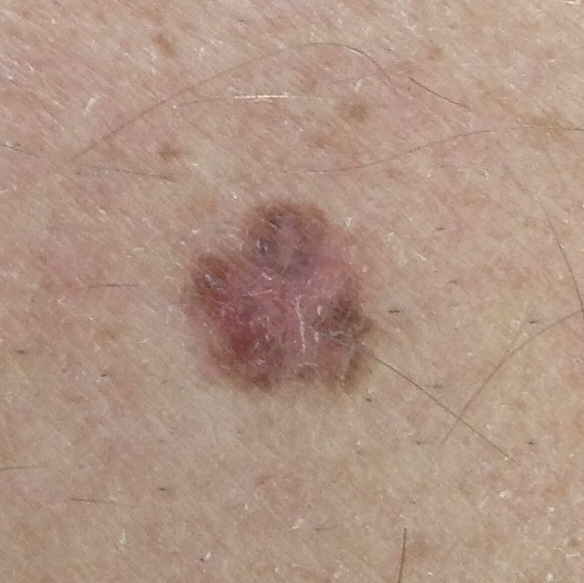
\includegraphics[width=.29\textwidth]{original.jpg}}
\qquad
\subfloat[][\emph{3 clusters image}\label{fig:1_2}]
{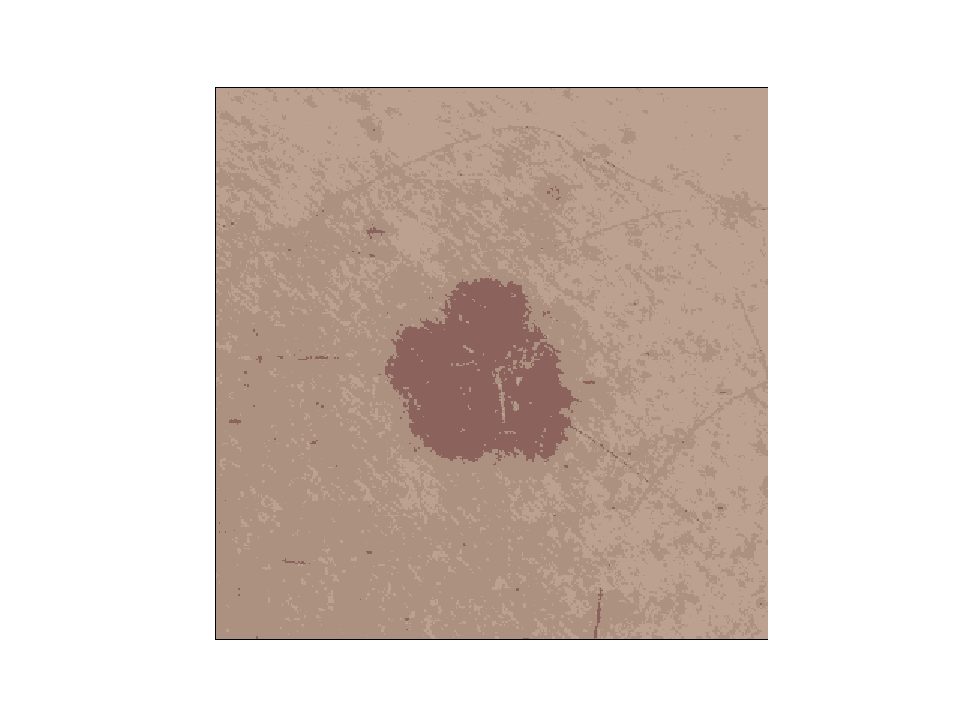
\includegraphics[width=.29\textwidth]{clusters.pdf}}
\qquad
\subfloat[][\emph{Centered binary image}\label{fig:1_3}]
{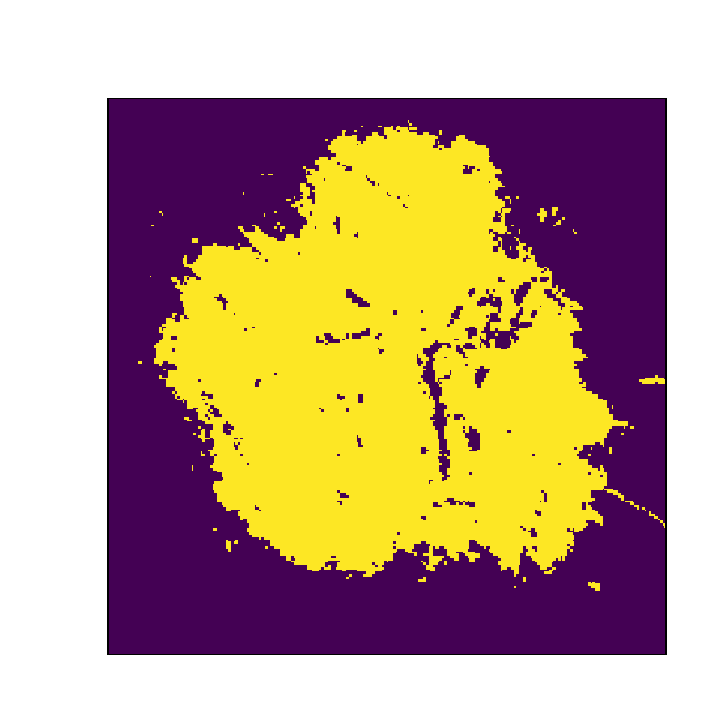
\includegraphics[width=.29\textwidth]{binary.pdf}}
\caption{Conversion of a photo into a binary image with a final centralization}
\label{fig:dataset1} 
\end{figure}


\chapter{Description of the algorithm}

\section{Image finishing}\label{sec:2_1}

\begin{wrapfloat}{figure}{R}{0pt}
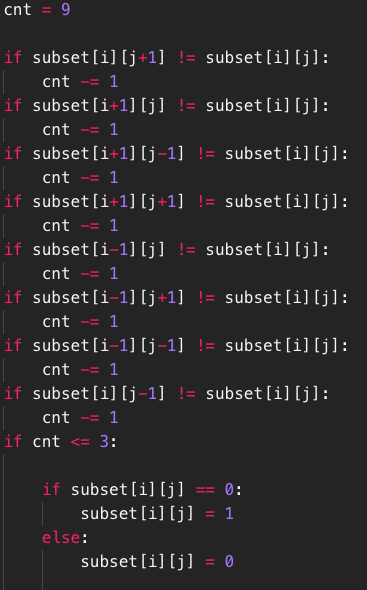
\includegraphics[width=0.25\textwidth]{clean.png}
\caption{Core of the cleaning algorithm}
\label{fig:dataset2} 
\end{wrapfloat}

First of all, the algorithm eliminates the noise from the binary image: the noise consists in a number of scattered pixels that are not useful to outline the shape of the mole. The binary image used is a matrix called \texttt{subset} (see figure [\textbf{\ref{fig:dataset2}}]) made of 0's [\textit{purple}] and 1's [\textit{yellow}]. We cancel the noise by analyzing, pixel by pixel, which value is more likely to recur, according to the nearest pixels. The key elements of this process are an initialized counter (\texttt{cnt = 9}) and the 8 nearest pixels that surround the pixel that is being analyzed. Every time a pixel near the one we are focusing on is different, the counter is decreased by one and if it goes down to 3, the pixel color is inverted (the number 3 is considered to be the threshold). Below in figure [\textbf{\ref{fig:dataset3}}] we can see the "before and after" the cleaning process; we still need to eliminate the holes and "islands" that surround the main element of the image. To do so, we will use an approach similar to the one we have just illustrated, as we will see in section [\textbf{\ref{sec:2_2}}]

\begin{figure}[h]
\centering
\subfloat[][\emph{Binary image}\label{fig:2_1}]
{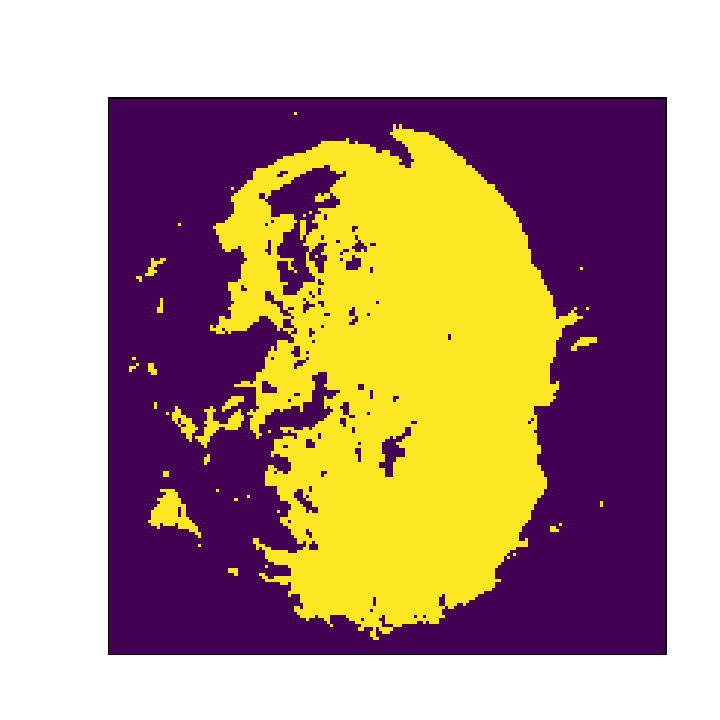
\includegraphics[width=.22\textwidth]{1_2a.pdf}}
\qquad
\subfloat[][\emph{Noiseless version}\label{fig:2_2}]
{
\includegraphics[width=.22\textwidth]{1_2b.pdf}}
\caption{Cleaning of the image's noise}
\label{fig:dataset3} 
\end{figure}


\section{Filling holes and eliminating the "islands"}\label{sec:2_2}

The algorithm is based on the same principle of the one in section [\textbf{\ref{sec:2_1}}], however we will examine the matrix in a different way and we will refer to a lower threshold in the counter for the conversion of a pixel's color. We will start by examining each quarter of the image, from the centre to the opposite angle (islands elimination) and vice-versa (holes filling) (see figure [\textbf{\ref{fig:2_5}}]). For the islands elimination we start exploring from out of the mole's shape taking for granted that portions of yellow pixels, found during the process, have to be considered "islands" and so, in need for a conversion. The same idea comes handy for filling the holes but this time we start examining the image from the centre, taking for granted that portions of purple pixels need to be converted. The conversion is always made by counting what is the color majority around the pixel in analysis but this time we set less "hard" conditions by initializing the counter equal to 8 and the threshold equal to 4, doing so we are able to convert bigger areas.



\begin{figure}[H]
\centering
\subfloat[][\emph{Directions of exploration}\label{fig:2_5}]
{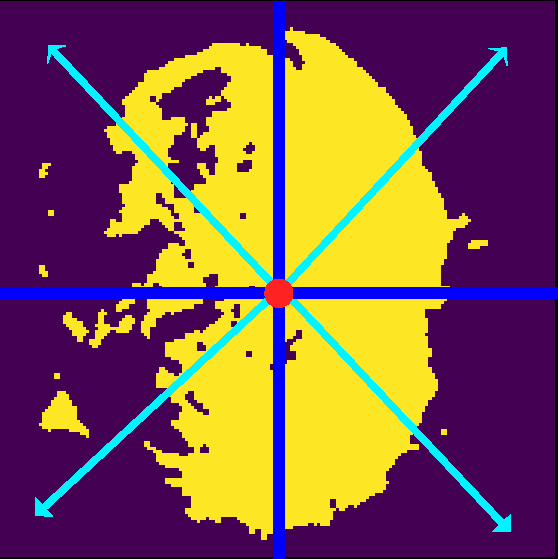
\includegraphics[width=.18\textwidth]{arrow.pdf}}
\qquad
\subfloat[][\emph{\scriptsize Final result}\label{fig:2_6}]
{
\includegraphics[width=.18\textwidth]{1_3.pdf}}\\
\caption{Image result}
\label{fig:dataset5} 
\end{figure}



\section{Finding the image perimeter}

\begin{wrapfloat}{figure}{R}{0pt}
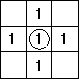
\includegraphics[width=0.11\textwidth]{str.png}
\caption{Structuring element}
\label{fig:dataset6} 
\end{wrapfloat}

For the perimeter we have used a very simple approach. With the aid of a structuring element such as the one in figure [\textbf{\ref{fig:dataset6}}], we will check each $3\times3$ section of the \texttt{subset[i][j]} and verify if the central pixel, the circled one in figure [\textbf{\ref{fig:dataset6}}], is surrounded by 4 other ones; if so, the central one (\textit{yellow}), becomes a 0 (\textit{purple}). The calculation of the perimeter and of the area of the mole is made by simply counting the ones in the binary image. The perimeter of the equivalent circle, with the same area, is given by the formula [\textbf{\ref{eq:1}}].
\\
\begin{equation}\label{eq:1}
\centering
Perimeter_{circle}=2\sqrt{\pi\cdot Area_{mole}} 
\end{equation}
\\
The final process consists in determining the ratio between the perimeter of the mole and the perimeter of the circle with the same area of the binary image.

\pagebreak


\section{Result examples}
The figures below ([\textbf{\ref{fig:dataset8}}], [\textbf{\ref{fig:dataset9}}] and [\textbf{\ref{fig:dataset10}}]) are an example of each mole category.
The video shows an animation of the proposed algorithm: \href{https://youtu.be/jqscD-K-eMs}{\underline{YouTube}} 

\begin{figure}[H]
\centering
\subfloat[][\emph{Photo}\label{fig:2_7}]
{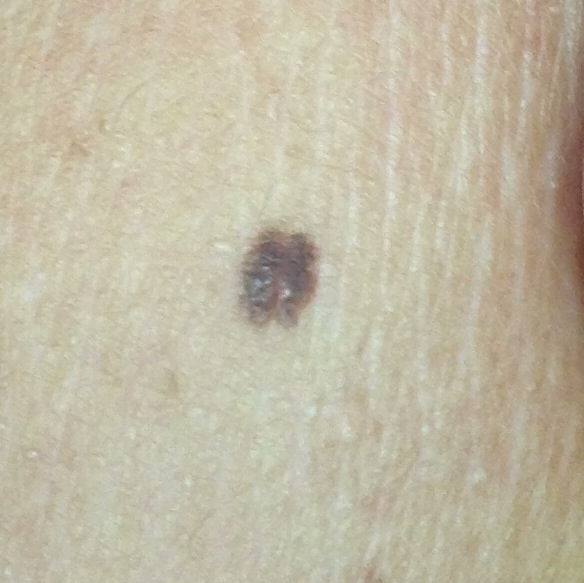
\includegraphics[width=.17\textwidth]{a1.jpg}}
\qquad
\subfloat[][\emph{Raw image}\label{fig:2_8}]
{
\includegraphics[width=.17\textwidth]{z1.pdf}}
\qquad
\subfloat[][\emph{Clean image}\label{fig:2_9}]
{
\includegraphics[width=.17\textwidth]{a2.pdf}}
\qquad
\subfloat[][\emph{Perimeter}\label{fig:2_10}]
{
\includegraphics[width=.17\textwidth]{a3.pdf}}
\caption{low\_risk\_mole\_4}
\label{fig:dataset8}

\subfloat[][\emph{Photo}\label{fig:2_11}]
{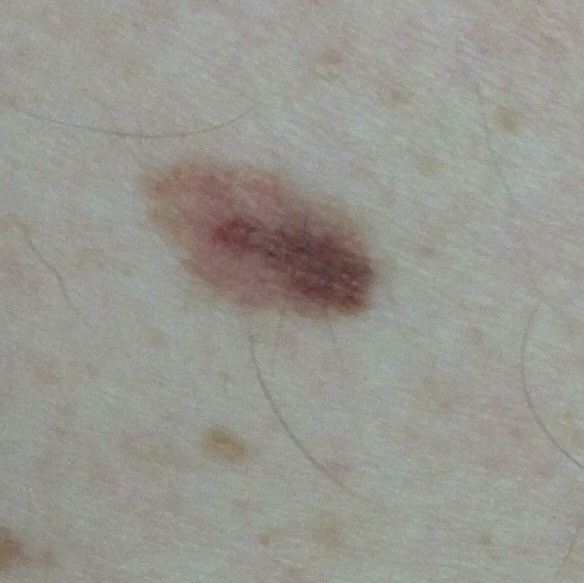
\includegraphics[width=.17\textwidth]{b1.jpg}}
\qquad
\subfloat[][\emph{Raw image}\label{fig:2_12}]
{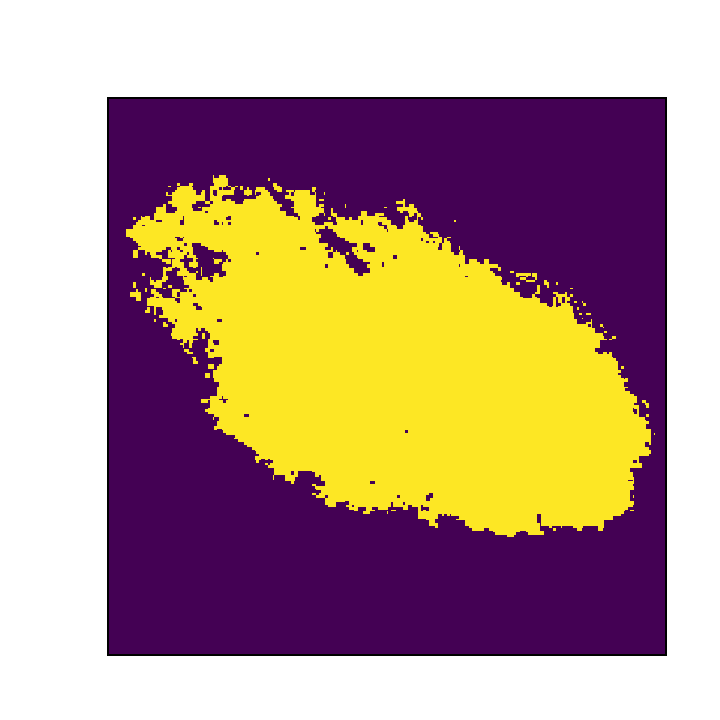
\includegraphics[width=.17\textwidth]{z2.pdf}}
\qquad
\subfloat[][\emph{Clean image}\label{fig:2_13}]
{
\includegraphics[width=.17\textwidth]{b2.pdf}}
\qquad
\subfloat[][\emph{Perimeter}\label{fig:2_14}]
{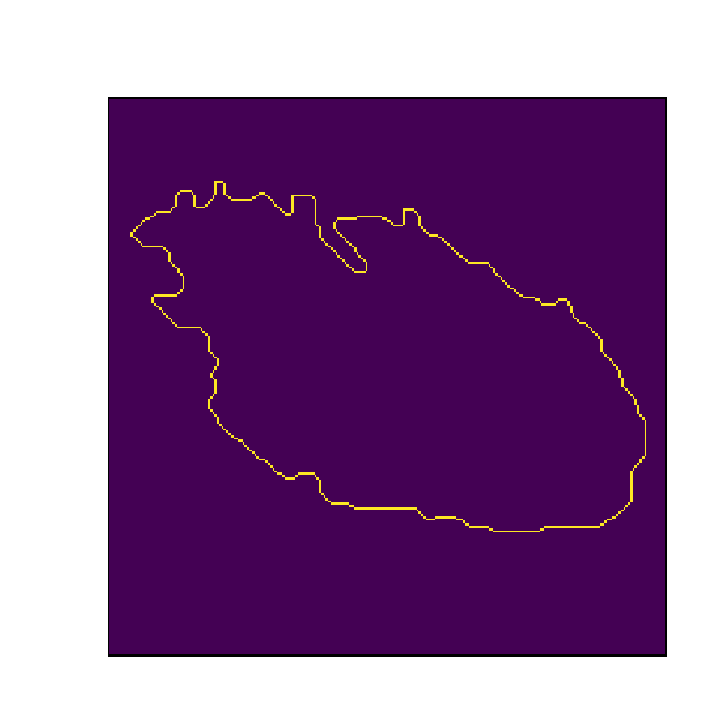
\includegraphics[width=.17\textwidth]{b3.pdf}}
\caption{medium\_risk\_mole\_5}
\label{fig:dataset9}

\subfloat[][\emph{Photo}\label{fig:2_15}]
{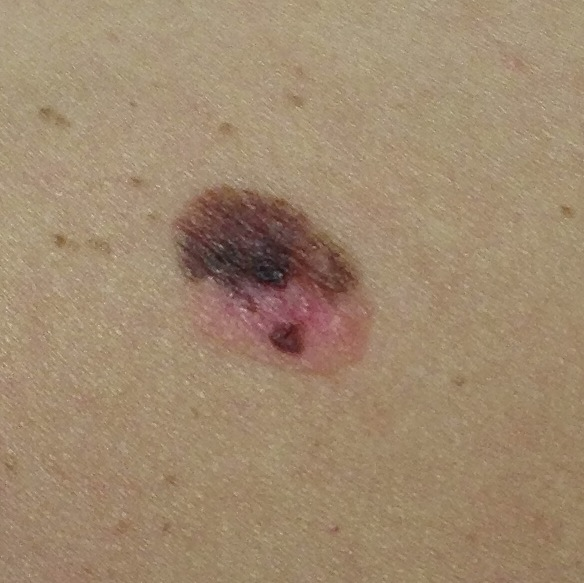
\includegraphics[width=.17\textwidth]{c1.jpg}}
\qquad
\subfloat[][\emph{Raw image}\label{fig:2_16}]
{
\includegraphics[width=.17\textwidth]{z3.pdf}}
\qquad
\subfloat[][\emph{Clean image}\label{fig:2_17}]
{
\includegraphics[width=.17\textwidth]{c2.pdf}}
\qquad
\subfloat[][\emph{Perimeter}\label{fig:2_18}]
{
\includegraphics[width=.17\textwidth]{c3.pdf}}
\caption{melanoma\_17}
\label{fig:dataset10} 
\end{figure}





\section{Data Results and comments}
The ratios obtained are shown in table [\textbf{\ref{table1}}]. An analysis of the results clearly reveals that the border alone is not sufficient to categorize the moles, as some numbers overlap between categories. However, there could be a correlation between the border’s indentation and the presence of skin cancer, as ratios are generally higher in case of melanomas than in case of low and medium risk moles. The mole \textit{low\_risk\_4} (figure [\textbf{\ref{fig:dataset8}}]), with a ratio of 1.043 (very close to the average ratio of medium risk moles in table [\textbf{\ref{table2}}]), could in all likelihood belong to the medium risk category; therefore it is evident that the border was not the only criterion used to categorize it. The same could be said for the mole \textit{medium\_risk\_5} (figure [\textbf{\ref{fig:dataset9}}]), whose ratio is 1.266, higher than the mean value of the melanomas (see table [\textbf{\ref{table2}}]). Figure [\textbf{\ref{fig:dataset10}}] shows \textit{melanoma\_17} (figure [\textbf{\ref{fig:dataset10}}]), whose border is rather irregular, consistently with its ratio of 1.509.
Finally, we can state that the evaluation of a mole’s perimeter and the computation of its ratio with a circumference of the same area is a useful instrument when combined with the other four criteria of the "ABCDE" method and, of course, with a medical examination.


\begin{table}[ht]\footnotesize
\begin{minipage}[b]{0.5\linewidth}%\centering
\begin{tabular}{|c|c|c|c|}
\hline
 \textbf{Image}  & \textbf{Mole} & \textbf{Circle} & \textbf{Ratio} \\
\hline
low\_risk\_1                          &326                     &326.68         &0.997\\
low\_risk\_2                          &327                     &360.34         &0.935\\
low\_risk\_3                          &281                     &254.19         &1.105\\
low\_risk\_4                          &273                     &261.53         &1.043\\
low\_risk\_5                          &252                     &246.87         &1.020\\
low\_risk\_6                          &278                     &287.74		    &0.966\\
low\_risk\_7                          &215                     &195.09	     	&1.102\\
low\_risk\_8                          &324                     &301.27	 		&1.075\\
low\_risk\_9                          &184                     &203.29         &0.905\\
low\_risk\_10                         &129                     &138.65         &0.930\\
low\_risk\_11                         &192                     &202.83	        &0.946\\
medium\_risk\_1                       &117						&128.84			&0.908\\
medium\_risk\_2                       &323						&333.57			&0.968\\
medium\_risk\_3                       &160						&169.30			&0.945\\
medium\_risk\_4                       &183						&185.18			&0.988\\
medium\_risk\_5                       &651						&513.98			&1.266\\
medium\_risk\_6                       &357						&315.11			&1.132\\
medium\_risk\_7                       &671						&636.05			&1.054\\
medium\_risk\_8                       &429		                &419.49			&1.022\\
medium\_risk\_9                       &295						&235.72			&1.251\\
medium\_risk\_10                      &421		                &388.51			&1.083\\
medium\_risk\_11                   	  &608		                &591.37			&1.028\\
medium\_risk\_12                      &405		                &432.27			&0.936\\
medium\_risk\_13                      &293		                &291.26			&1.005\\
medium\_risk\_14                      &336		                &349.65			&0.960\\
medium\_risk\_15                      &325		                &320.75			&1.013\\
medium\_risk\_16                      &471		                &483.03			&0.975\\
\hline
\end{tabular}
\end{minipage}
\hspace{0.6cm}
\begin{minipage}[b]{0.1\linewidth}
\centering
\begin{tabular}{|c|c|c|c|}
\hline
 \textbf{Image}  & \textbf{Mole} & \textbf{Circle} & \textbf{Ratio} \\
 \hline
melanoma\_1                         &396	 &392.07	 &1.010\\
melanoma\_2                         &335	 &312.97	 &1.070\\
melanoma\_3                         &460	 &353.35	 &1.301\\
melanoma\_4                         &472	 &400.43 &1.178\\
melanoma\_5                         &472	 &356.15	 &1.325\\
melanoma\_6                         &982	 &773.31	 &1.269\\
melanoma\_7                         &726	 &697.93	 &1.040\\
melanoma\_8                         &523	 &429.46	 &1.217\\
melanoma\_9                         &728	 &570.98	 &1.274\\
melanoma\_10                        &619	 &573.45	 &1.079\\
melanoma\_11                        &500	 &446.40	 &1.120\\
melanoma\_12                        &582	 &584.82	 &1.195\\
melanoma\_13                        &559	 &471.53	 &1.185\\
melanoma\_14                        &438	 &421.08	 &1.040\\
melanoma\_15                        &573	 &485.92	 &1.179\\
melanoma\_16                        &450	 &388.21	 &1.159\\
melanoma\_17                        &663	 &439.23	 &1.509\\
melanoma\_18                        &700	 &723.07	 &1.368\\
melanoma\_19                        &565	 &534.37	 &1.057\\
melanoma\_20                        &730	 &652.42	 &1.118\\
melanoma\_21                        &475	 &373.88	 &1.270\\
melanoma\_22                        &461	 &460.42	 &1.001\\
melanoma\_23                        &1542&654.30 &2.356\\
melanoma\_24                        &797	 &659.74	 &1.208\\
melanoma\_25                        &293	 &295.27	 &1.292\\
melanoma\_26                        &498	 &444.72	 &1.119\\
melanoma\_27                        &306	 &237.77	 &1.286\\
\hline
\end{tabular}
\end{minipage}
\caption{Tables with the perimeter of the mole, of the equivalent circle and the ratio of the perimeters}
\label{table1}
\end{table}


\begin{table}[ht]\footnotesize
\centering
\begin{tabular}{|l|c|c|}
\hline
\multicolumn{1}{|c|}{\textbf{Image}} & \textbf{Average of the ratios} & \textbf{Standard deviation of the ratios} \\ \hline
Low Risk & 1,002181 & 0,0717 \\
Medium Risk & 1,033375 & 0,1044 \\
Melanoma & 1,197248 & 0,2646 \\ \hline
All categories & 1,108957 & 0,2155 \\ \hline
\end{tabular}
\caption{Average and Standard Deviation for each category of moles}
\label{table2}
\end{table}



\end{document}